\section{Модальное управление по выходу}
Рассмотрим систему: 
\begin{equation}
    \begin{cases}
        \dot{x} = Ax + Bu \\
        y = Cx + Du
    \end{cases}
\end{equation} 
где
\begin{equation}
    \begin{array}{cccc}
        A = \begin{bmatrix}
            6 & 0 & -12 & 6 \\ 
            0 & 6 & -6 & 12 \\
            -12 & -6 & 6 & 0 \\
            6 & 12 & 0 & 6
        \end{bmatrix}, & 
        B = \begin{bmatrix}
            6 \\ 12 \\ 6 \\ 4
        \end{bmatrix}, & 
        C = \begin{bmatrix}
            -6 & 6 & 6 & 6 \\
            3 & 0 & 0 & 3
        \end{bmatrix}, 
        D = \begin{bmatrix}
            2 \\ 2
        \end{bmatrix}
    \end{array}
\end{equation}

\subsection{Система с регулятором и наблюдателем}
Рассмотрим систему с регулятором и наблюдателем:
\begin{equation}
    \begin{array}{ll}
        \hat{x} = A\hat{x} + (B + LD)u + L(C\hat{x} - y)\\
        u = K\hat{x}
    \end{array}
\end{equation}
И составим ее схему моделирования (см. рисунок \ref{fig:scheme3}).
\begin{figure}[ht!]
    \centering
    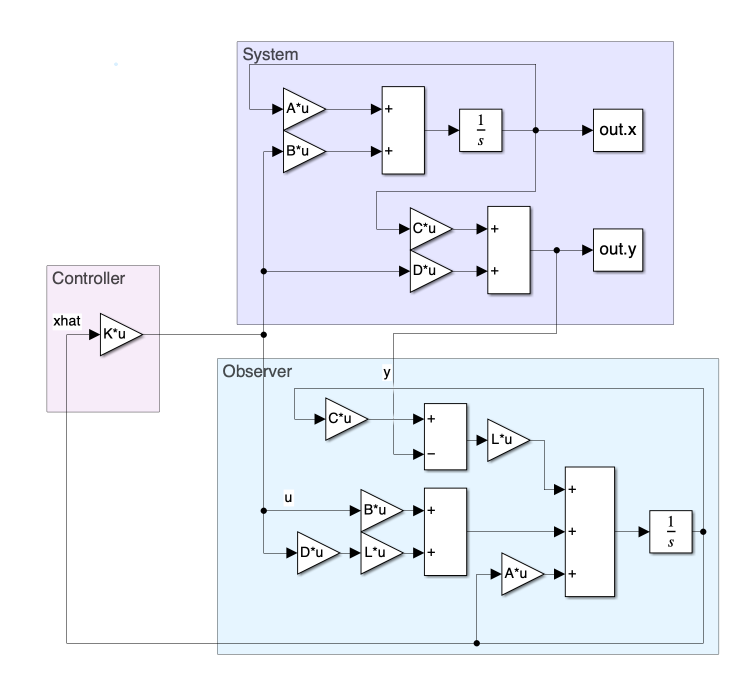
\includegraphics[width=0.8\textwidth]{media/scheme3.png}
    \caption{Схема моделирования системы с регулятором и наблюдателем}
    \label{fig:scheme3}
\end{figure}

\subsection{Управляемость и наблюдаемость}

Для определения управляемости и наблюдаемость собственных чисел рассмотрим вещественную Жорданову форму системы:
\begin{equation}
    \begin{cases}
        \dot{\hat{x}} = P^{-1}AP\hat{x} + P^{-1}Bu \\
        \hat{y} = C\hat{x} + Du
    \end{cases}
\end{equation}
\begin{equation}
    \begin{array}{cccc}
        A_j = \begin{bmatrix}
            0.00  & 0.00  & 0.00  & 0.00 \\ 
            0.00  & 12.00  & 0.00  & 0.00 \\ 
            0.00  & 0.00  & -12.00  & 0.00 \\ 
            0.00  & 0.00  & 0.00  & 24.00 \\ 
            \end{bmatrix}, &
        P = \begin{bmatrix}
            1.00  & -1.00  & -1.00  & 1.00 \\ 
            -1.00  & 1.00  & -1.00  & 1.00 \\ 
            1.00  & 1.00  & -1.00  & -1.00 \\ 
            1.00  & 1.00  & 1.00  & 1.00 \\ 
            \end{bmatrix}, \\
        B_j = \begin{bmatrix}
            1.00 \\ 
            4.00 \\ 
            -5.00 \\ 
            4.00 \\ 
            \end{bmatrix}, & 
        C_j = \begin{bmatrix}
            0.00  & 24.00  & 0.00  & 0.00 \\ 
            6.00  & 0.00  & 0.00  & 6.00 \\ 
        \end{bmatrix}
    \end{array}
\end{equation}

Можно сделать вывод, что система является полностью управляемой, а 
а собственное число $\lambda_3 = -12$ не является наблюдаемым. Соответственно, 
система не является полностью наблюдаемой, но, так как собственное число 
$\lambda_3$ располагается в левой полуплоскости, то система является обнаруживаемой. 

\subsection{Регулятор}
Выберем спектр регулятора равным $\{-4, -1, -2, -3\}$. Данный спектр является достижимым, 
так как не содержит неуправляемых собственные чисел. 

Аналогично первому заданию выберем матрицу $K$ таким образом, чтобы спектр матрицы $A - BK$
совпадал со спектром регулятора.
\begin{equation}
    K = \begin{bmatrix}
        -3.72  & -2.13  & 3.79  & -2.21 \\ 
    \end{bmatrix}
\end{equation}
При этом, как и ожидалось, спектр матрицы $A - BK$ полностью совпадает с желаемым спектром регулятора.

\subsection{Наблюдатель}
Выберем спектр наблюдателя равным $\{-1, -2, -3, -12\}$. Данный спектр является достижимым,
так как содержит не наблюдаемое собственное число $\lambda_3 = -12$.

Аналогично второму заданию выберем матрицу $L$ таким образом, чтобы спектр матрицы $A - LC$
совпадал со спектром наблюдателя.
\begin{equation}
    L = \begin{bmatrix}
        -11.24  & -11.24 \\ 
        -9.65  & -9.65 \\ 
        10.66  & 10.66 \\ 
        -9.08  & -9.08 \\ 
    \end{bmatrix}
\end{equation}
При этом спектр матрицы $A - LC$ полностью совпадает с желаемым спектром наблюдателя.

\subsection{Моделирование}
Промоделируем систему с регулятором и наблюдателем с начальными условиями $x(0) = [1, 1, 1, 1]^T$ и $\hat{x}(0) = [0, 0, 0, 0]^T$. 
Результаты моделирования представлены на рисунках \ref{fig:task3_x} (состояние системы) и \ref{fig:task3_xhat} (оценка состояния системы) и 
\ref{fig:task3_u} (управляющее воздействие). График ошибки оценки состояния представлен на рисунке \ref{fig:task3_diff}.

\begin{figure}[ht!]
    \centering
    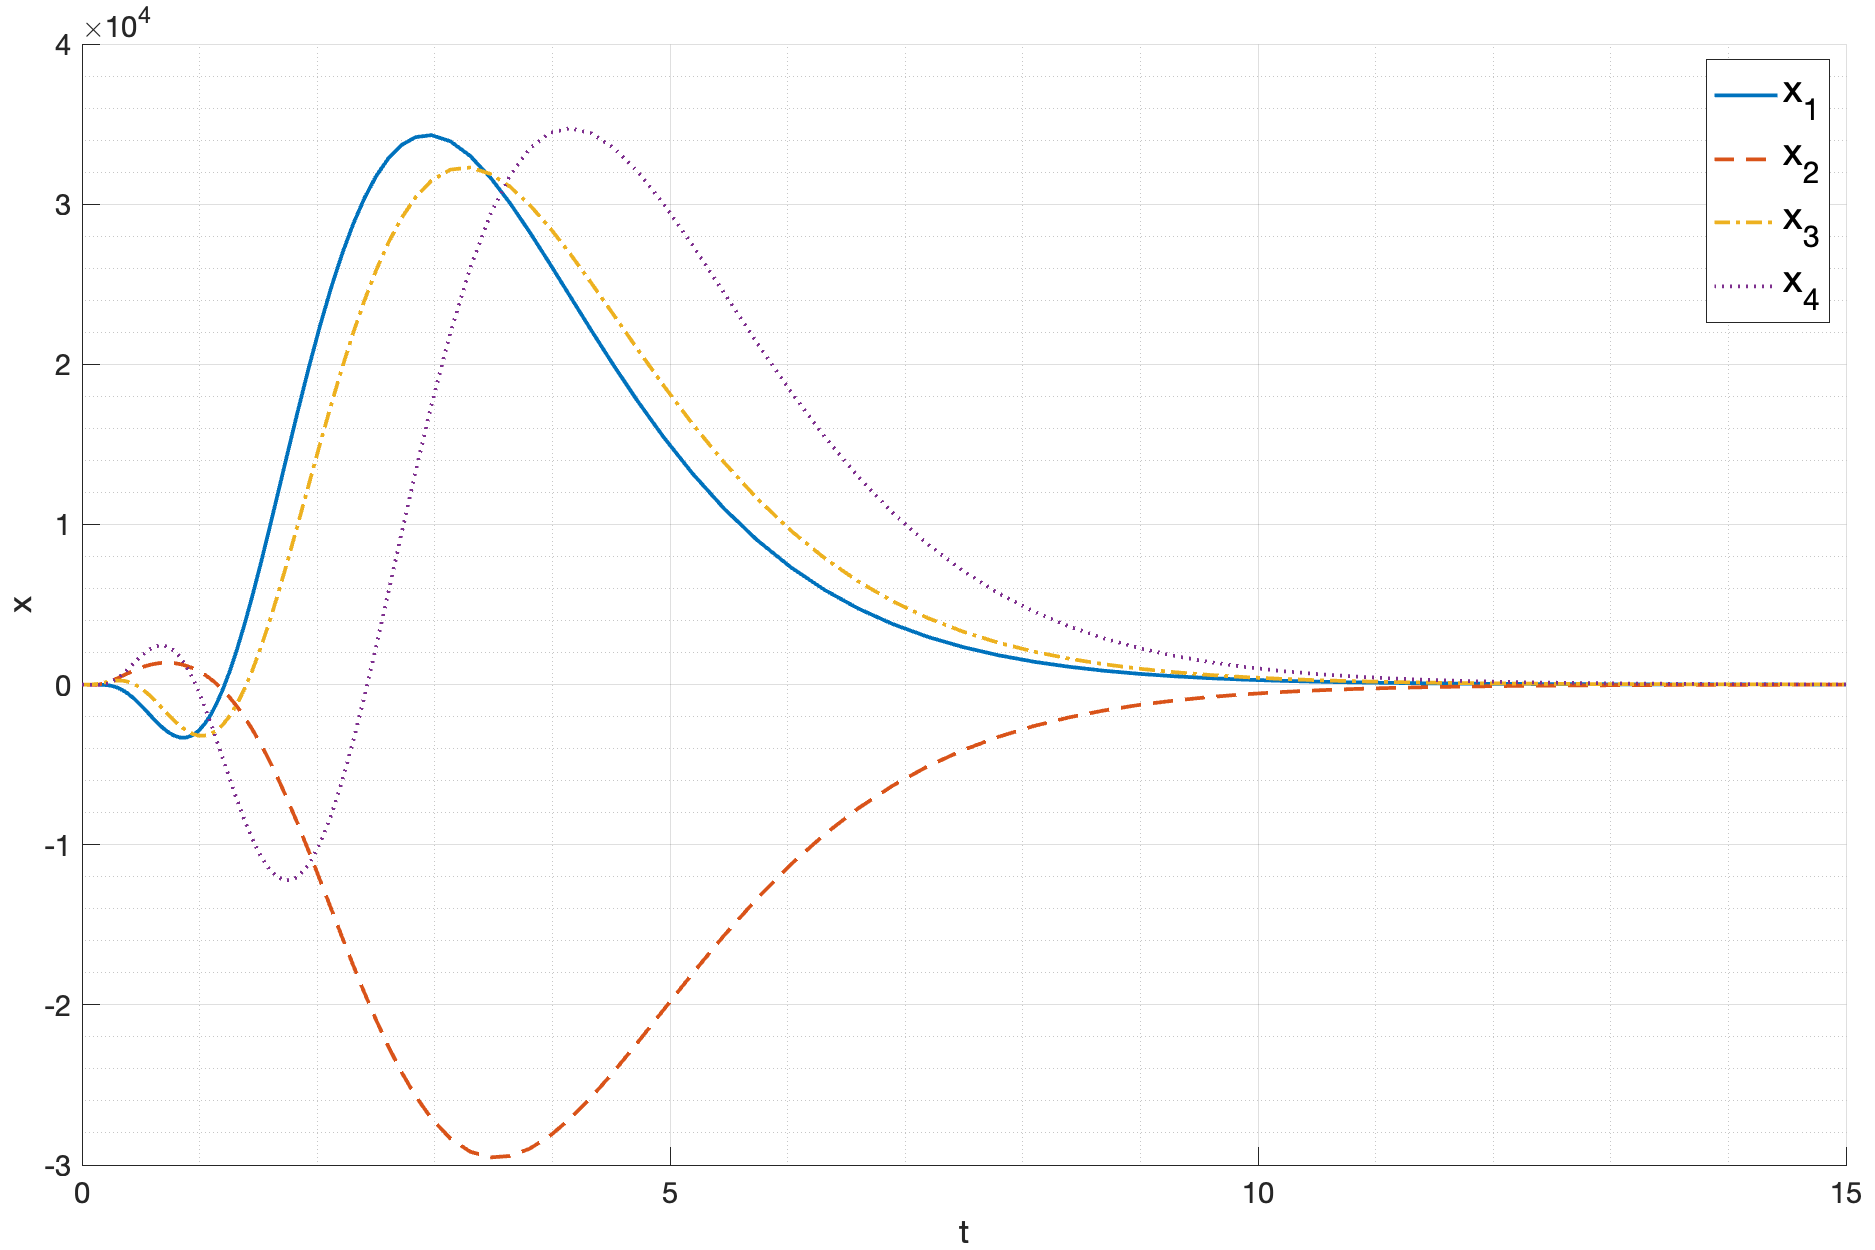
\includegraphics[width=0.8\textwidth]{media/plots/task3_x_1.png}
    \caption{Состояние системы}
    \label{fig:task3_x}
\end{figure}

\begin{figure}[ht!]
    \centering
    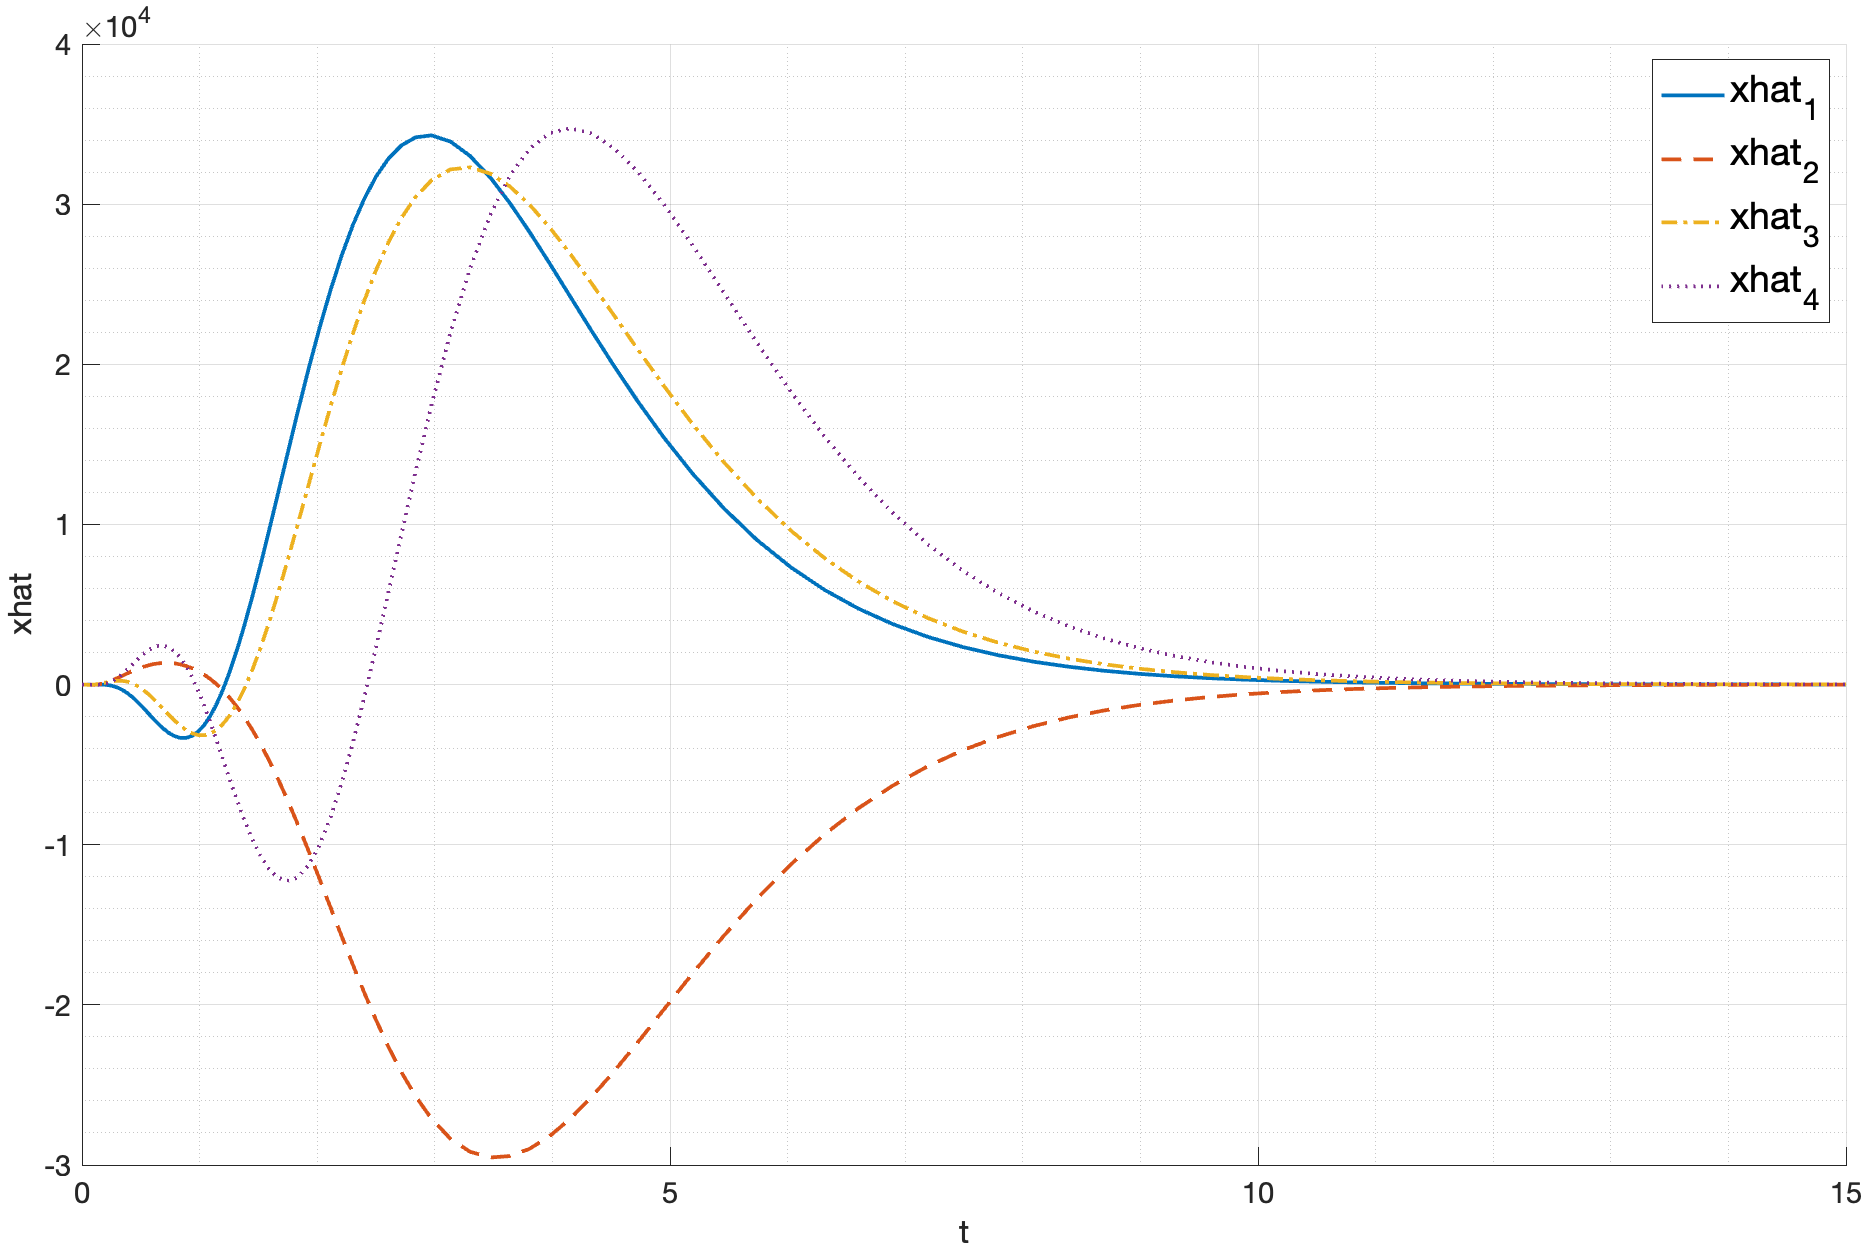
\includegraphics[width=0.8\textwidth]{media/plots/task3_xhat_1.png}
    \caption{Оценка состояния системы}
    \label{fig:task3_xhat}
\end{figure}

\begin{figure}[ht!]
    \centering
    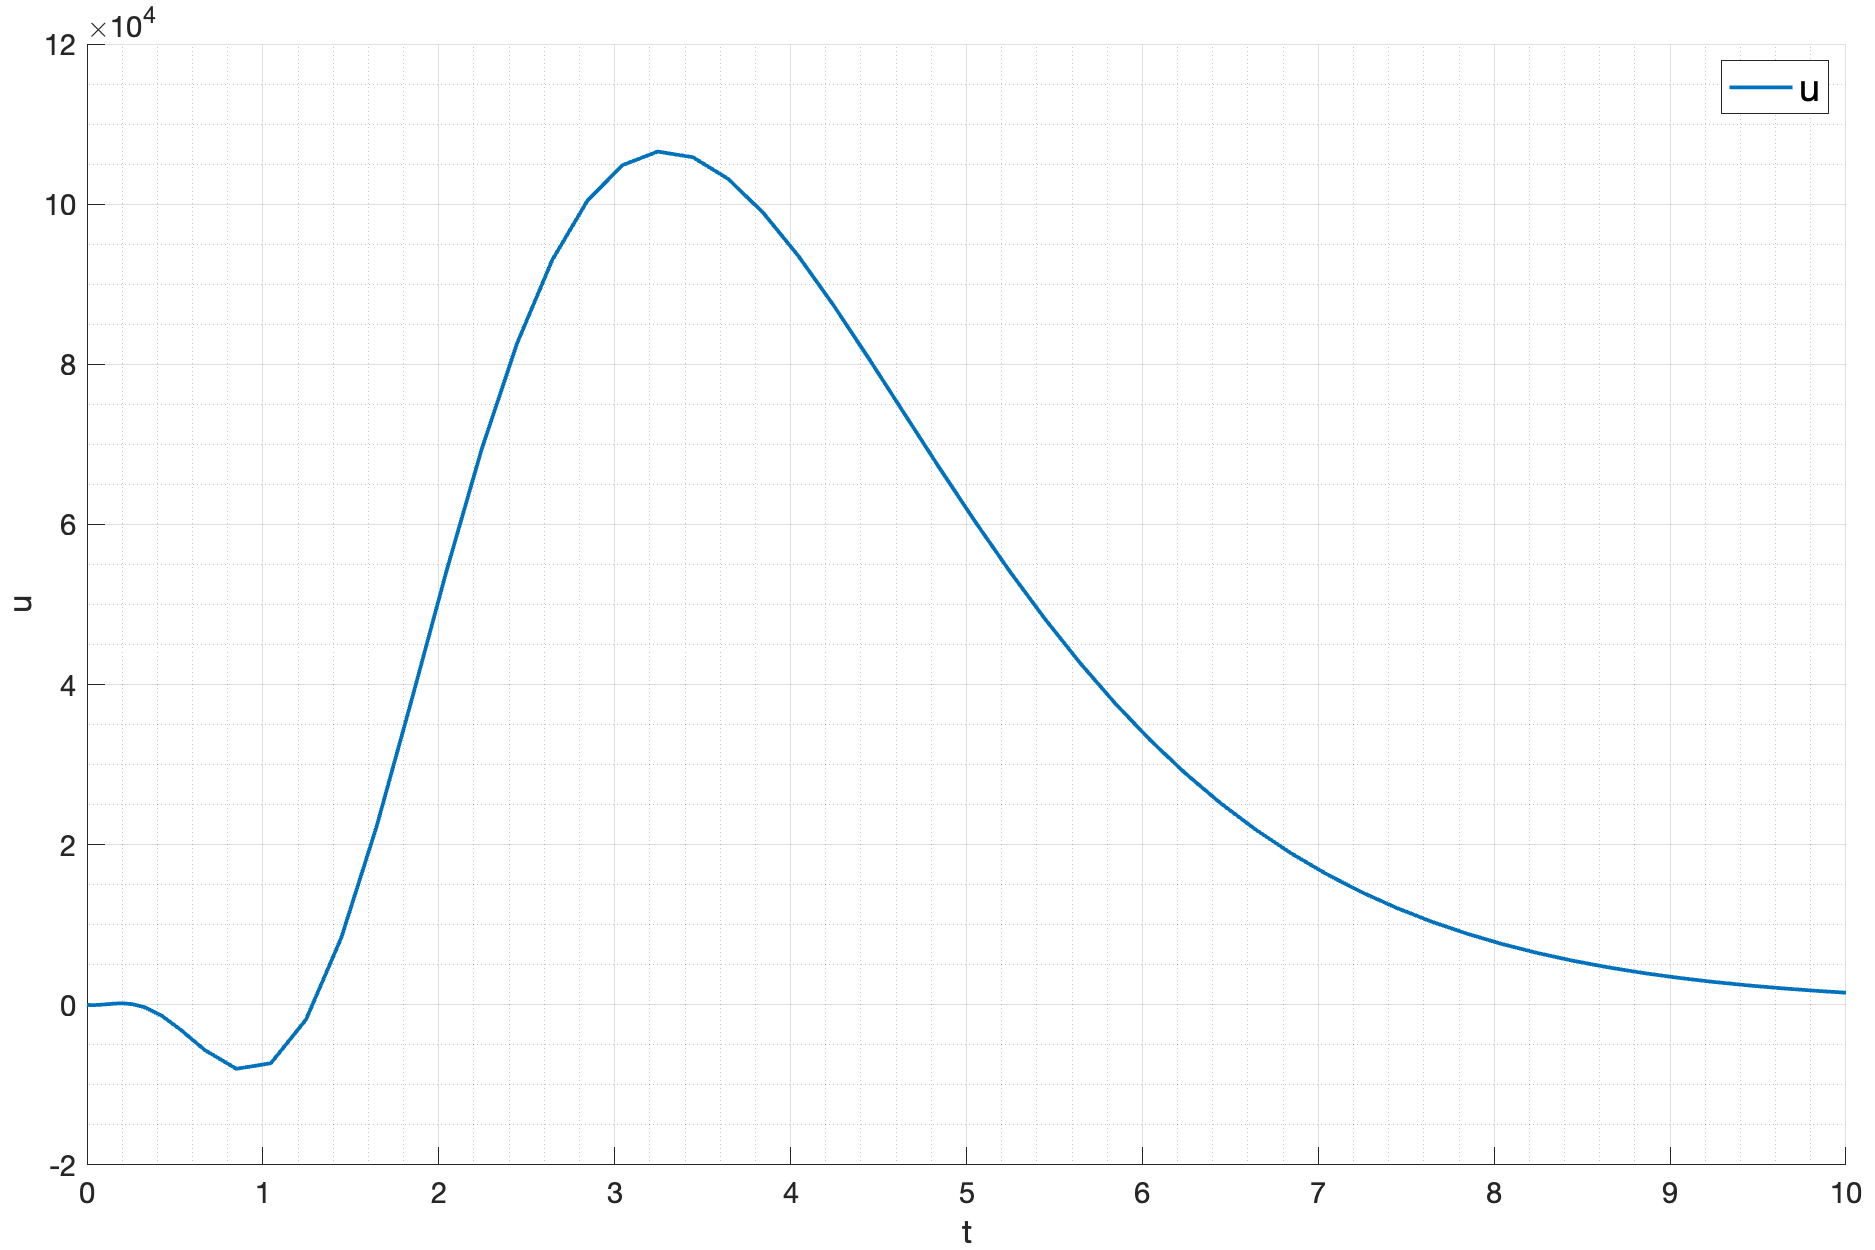
\includegraphics[width=0.8\textwidth]{media/plots/task3_u_1.png}
    \caption{Управляющее воздействие}
    \label{fig:task3_u}
\end{figure}

\begin{figure}[ht!]
    \centering
    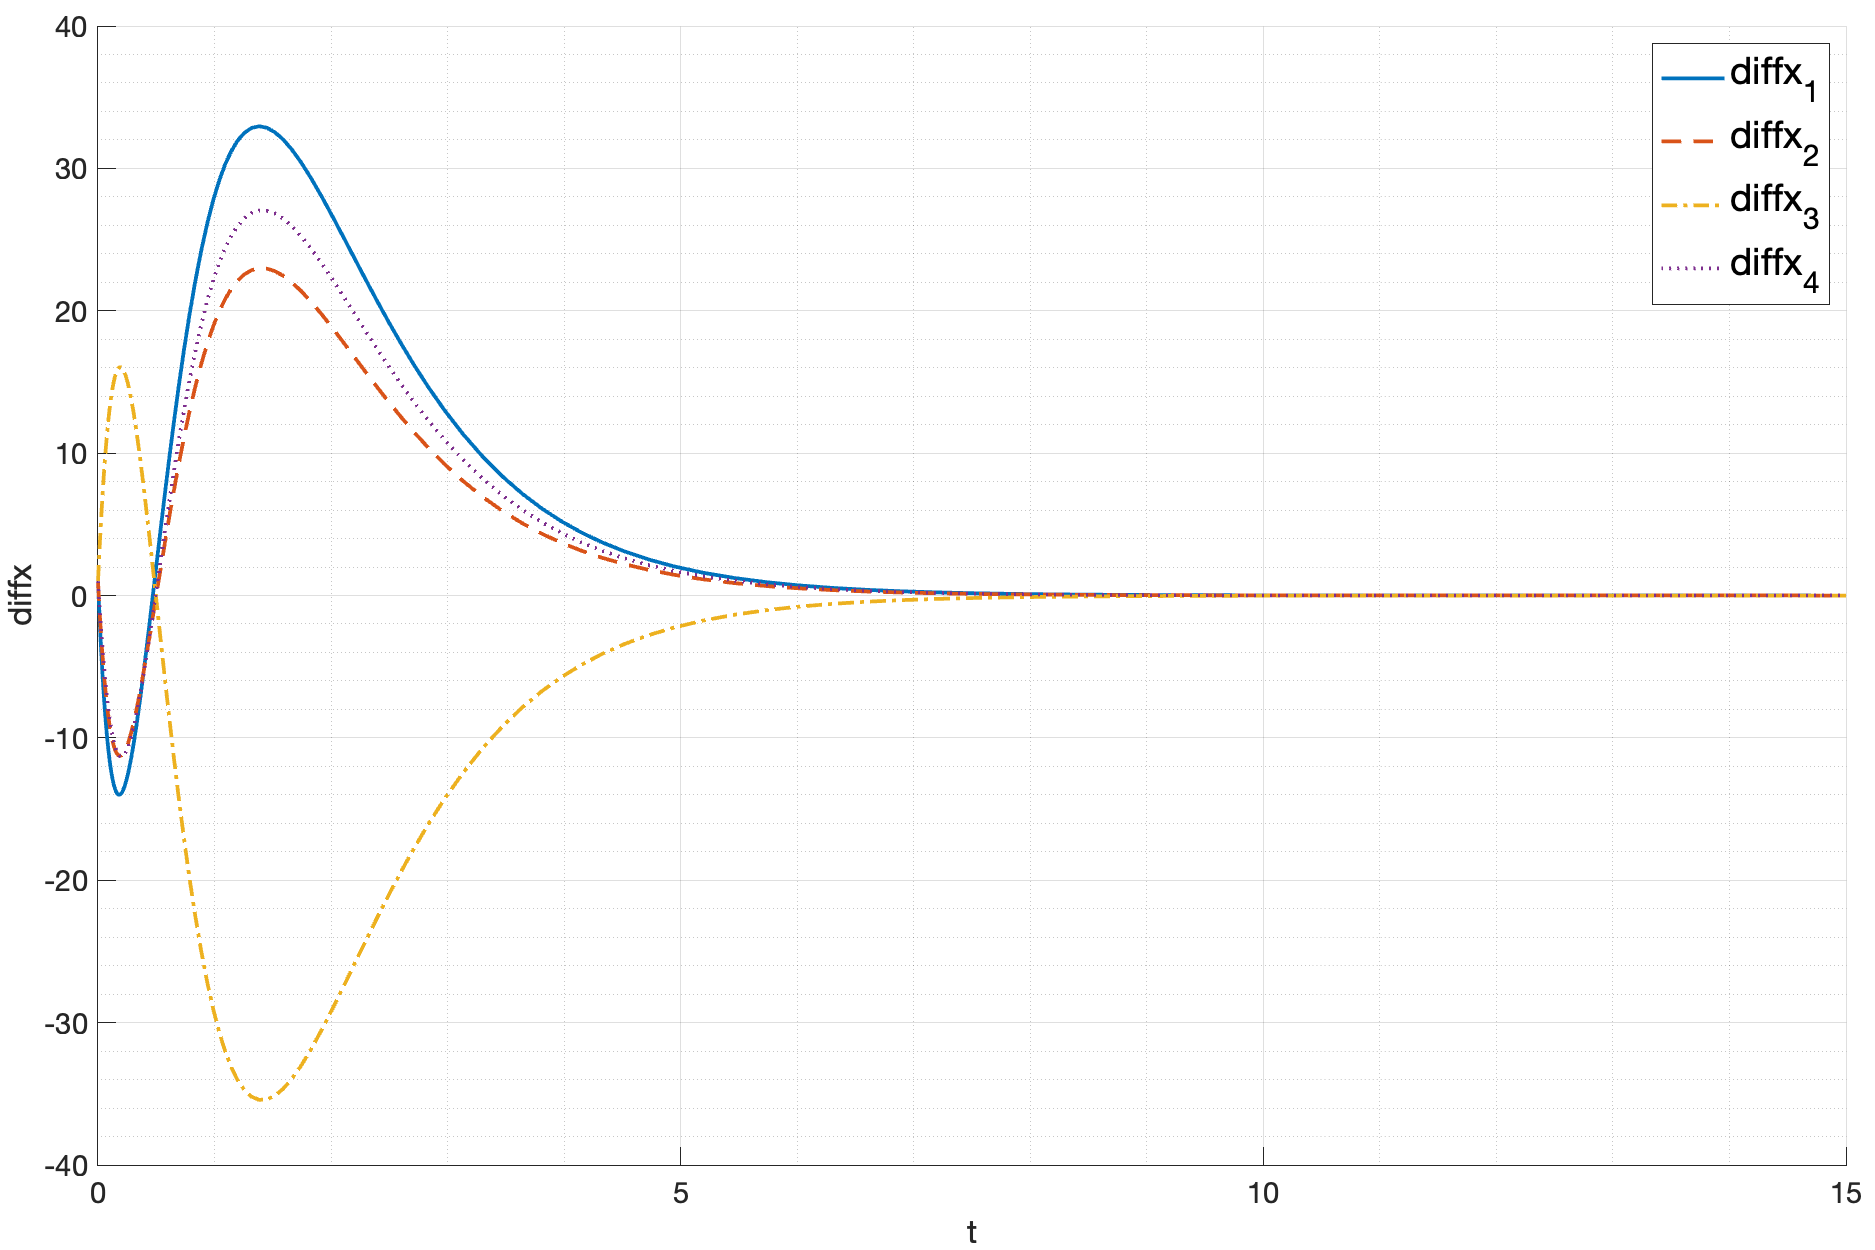
\includegraphics[width=0.8\textwidth]{media/plots/task3_diffx_1.png}
    \caption{Ошибка оценки состояния}
    \label{fig:task3_diff}
\end{figure}

\FloatBarrier
\subsection{Выводы}
В результате моделирования системы с регулятором и наблюдателем можно сделать вывод, что регулятор, основанный 
на оценке состояния системы, позволяет управлять системой так же, как и регулятор, основанный на реальном
состоянии системы. При этом, ошибка оценки состояния системы быстро сходится к нулю. 